\documentclass{tdk_style}
\usepackage{fullpage}

\author{\href{mailto:balint.balazs@molbiol.eu}{Bálint Balázs}}
\supervisor{\href{mailto:hufnagel@embl.de}{Lars Hufnagel}}
\lab{\href{http://www.embl.de/}{European Molecular Biology Laboratory}}
\university{\href{http://www.ppke.hu/}{Pázmány Péter Catholic University}}
\collegeordept{\href{http://www.itk.ppke.hu/}{Faculty of Information Technology} \\ Infobionics MSc, 2\textsuperscript{nd} semester}
\degreedate{November, 2012}
\ppke{
\includegraphics[width=2cm]{figures/0_front/ITK_logo}}
\embl{\includegraphics[width=5cm]{figures/0_front/EMBL_logo}}
\degree{TDK}

\title{Development of a symmetric single-plane illumination microscope}
%\date{2012 november}
\begin{document}

\maketitle

\begin{abstract}
To better understand development of complex biological systems, imaging of living samples over time is necessary. Using the light-sheet based Single-Plane Illumination Microscopy (SPIM), it became possible to image live specimens with high resolutions in 3 dimensions over time. Fast image acquisitions makes cell tracking possible even in highly motile samples, such as a developing drosophila embryo, zebrafish brain, or phallusia embryo. 

This microscopy technique uses two perpendicularly aligned objectives. One is used to illuminate a thin plane of the specimen, and the other is used to capture an image of this plane. Compared to confocal microscopy, this method provides better 3D resolution, higher acquisition rate and less phototoxicity. This makes light-sheet based microscopy especially suitable for imaging live specimens over a long period of time.

The aim of this work is to build a SPIM that uses identical objectives, and uses both of them for illumination and detection in an alternating fashion. This will significantly improve 3D resolution, because the two images taken from different views can be fused together providing a better resolution than either of them.

To be able to control and automate the microscope, we also designed a custom program that controls image acquisition and handles user interactions. Our aim when developing this program was that it should be modular and easily adaptable to different kinds of SPIM setups.

Our final goal is to use this microscope to image live specimens. Using data acquired with this microscope it will be possible to segment cells, and track cell divisions and cell migrations. This will provide valuable information on embryonic development in several species.
\end{abstract}

\tableofcontents




\chapter{Introduction}
Vision is the most important of all of our senses, it provides the brain with more information than all the other senses together. However, using just the naked eye, it is not possible to answer all the questions of a curious mind. Using the tool of optics however, one can construct such instruments that allow to extend the boundaries of one's eyes, and see much farther, or much closer.

Microscopy, derived from the ancient Greek words mikros, ``small" and skopein, ``to see", aims to bring us closer to understand our world, by making it possible to visualise much smaller things than the naked eye can perceive.

Optical microscopy, or as often called, light microscopy uses a system of lenses to alter the path of visible light, and create magnified images of small samples. It dates back to the 17\textsuperscript{th} century, when Leeuwenhoek first observed single cells using carefully crafted glass spheres. It was also realized, that using multiple lenses, a more powerful device can be constructed.

Since then, optical microscopy advanced a great deal, and today it extended its boundaries to the infrared and ultraviolet range of light. The light source used for imaging is usually a light bulb, LED or laser. The path of the light is controlled by lenses, mirrors and apertures between the light source, the sample and the detection unit. The detection unit, if not our own eyes, can be a photomultiplier or a digital (CCD or sCMOS) camera.

Image appears on the detector, because the sample somehow interacts with the illumination light: it transmits, absorbs, reflects and scatters it. These can be visualized in different ways. Modern light microscopy also takes advantage of detecting all three properties of the light (wavelength, polarization and momentum), which provides us with a wide variety of different contrasts.

In this work I will first revise current light microscopy techniques, and in Chapter \ref{chap2} show the principles of single-plan illumination microscopy. In Chapter \ref{chap3} I describe a custom program that was developed to control and automate a SPIM microscope. Finally, in Chapter \ref{chap4} I demonstrate the capabilities of our symmetric SPIM controlled by the custom program.

\newpage

\section{Fluorescence microscopy}
Fluorescence microscopy \cite{lichtman_fluorescence_2005} is a microscopy technique that uses fluorophores, a special group  of chemicals that are capable of absorbing a photon of well defined energy, and emit a different photon within a stochastically determined time frame. The emitted photon usually has less energy than the absorbed photon, it is shifted towards the red side of the spectrum. This effect is called the Stokes-shift.

Using this phenomenon, it is possible to differentiate between the photons used for excitation and the emitted photons using an appropriate filter. Since the emitted photon usually has less energy, a low-pass filter can be used that will filter out the higher energy, lower wavelength illumination photons. Even though a very small amount of illumination photons will result in fluorescence ($<0.0001\%$), the signal to noise ratio of the fluorescence is still very high due to the filtering.

Fluorescent microscopy is especially suitable to image live specimens, since a lot of organisms has naturally fluorescent structures. This phenomenon is called autofluorescence.

Imaging specimens using just autofluorescence although can be useful in some cases, but in most of the time we would want to narrow our interest in a specific part, specific structure of the specimen. This can be achieved in several ways, but the simplest and earliest solution is the use of fluorescent dyes. These dyes, as the name implies, emit fluorescence under a certain excitation wavelength, and have such a structure, that they can specifically bind to certain parts of the cell. Fluorescent dyes although very useful in most cases, have some limitations. 

However, fluorescent microscopy took a great leap with the discovery of the green fluorescent protein. This had such an impact on future development of fluorescence microscopy, that three scientists were awarded with a Nobel Prize in chemistry in 2008 for it's discovery \cite{service_three_2008}. Since then, several variants were generated, and so today a whole spectrum of fluorescent proteins are available \cite{shaner_guide_2005}. The huge benefit of these proteins over the synthetic fluorescent dyes, is that the cell is capable of producing them by itself. Using genetic manipulation techniques, it is possible to introduce the genetic material coding a fluorescent protein into the genome of virtually any organism. These proteins can also be modified and fused with certain proteins of interest. Using this technique, the fluorescent protein will be attached to a functional protein, this way its expression and localisation pattern can be determined.

\subsection{Wide-field fluorescence microscopy}

One of the simplest fluorescent microscopes is a wide-field fluorescent microscope (Figure \ref{fig:wide-field}). The main difference to a regular microscope, is the introduction of a filter cube. This cube contains an excitation filter, emission filter and a dichroic mirror. The dichroic mirror is used to couple the illumination and detection light paths, and the filters are used to separate the fluorescent light from the excitation light. The image of the sample is focused on the detector of a digital camera.

\begin{figure}[htbp]
	\centering
	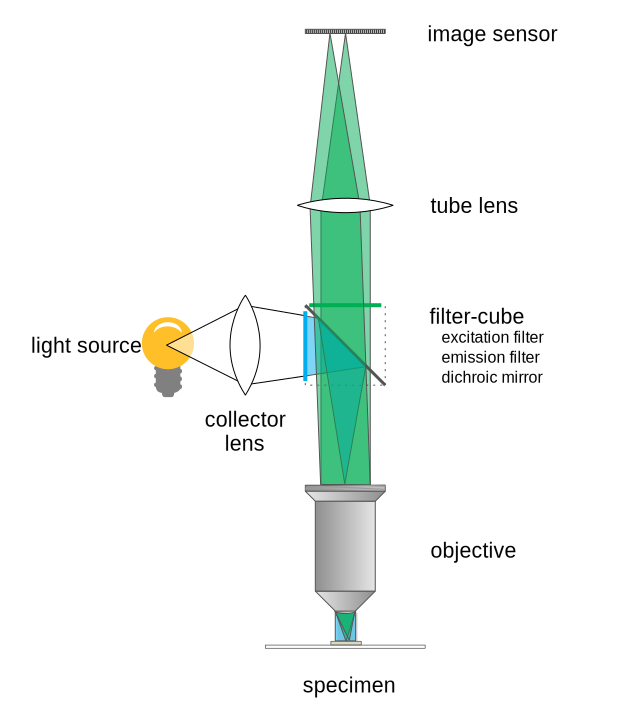
\includegraphics[scale=0.4]{figures/1_introduction/wide-field}
	\caption{\textbf{Wide-field fluorescent microscope.}}
	\label{fig:wide-field}
\end{figure}

\subsubsection{Resolution of a wide-field microscope}

Resolution of a microscope is given by the minimal distance of two point that can sill be distinguished. The smaller this distance is, the better the resolving power of the microscope. However, the resolution is limited by the wave nature of light, and cannot be decreased infinitely.

A generally accepted method to calculate lateral ($\sigma_{xy}$) and axial ($\sigma_{z}$) resolution of an optical microscope is described by the Stelzer-Grill-Heisenberg, or SGH theory\cite{grill_method_1999, stelzer_uncertainty_2000}:
\begin{equation} \label{eq:latres}
\sigma_{xy}=\frac{\lambda}{\sqrt{3-2 \cos \alpha - \cos 2 \alpha}}
\end{equation}
\begin{equation} \label{eq:axres}
\sigma_z = \frac{\lambda}{1-\cos \alpha}
\end{equation}
Generally, instead of $\alpha$, the numerical aperture (NA) is commonly used to characterize a lens' aperture. 
$NA=n\cdot \sin \alpha$, where n is the refractive index of the medium and $\alpha$ stands for the angular aperture.

Although high NA objectives have better axial resolution (Figure~\ref{fig:resolution}), this is still around 3--6 times worse than the lateral resolution. In theory, it is possible to achieve isotropic resolution in case of $\alpha = 180^\circ$, which means collecting all light emitted from the sample. However, it is currently unachievable to realize such a device that is capable of this. Because of this, 3D imaging with any microscopy technique that use one objective will always produce an anisotropic image.

Another disadvantage of the wide-field microscope, is that it can not be used with thick specimens. Usually this type of microscopy is only used for a single layer of cells, because all the objects in the field of view will appear on the imaging plane, not just the plane in focus. These objects will appear blurred if close to the focus, or just evenly add to the background noise if they are further from the focus. This is why imaging specimens much thicker than $10\ \mu m$ will result in suboptimal image quality.

\begin{figure}[htpb]
	\centering
	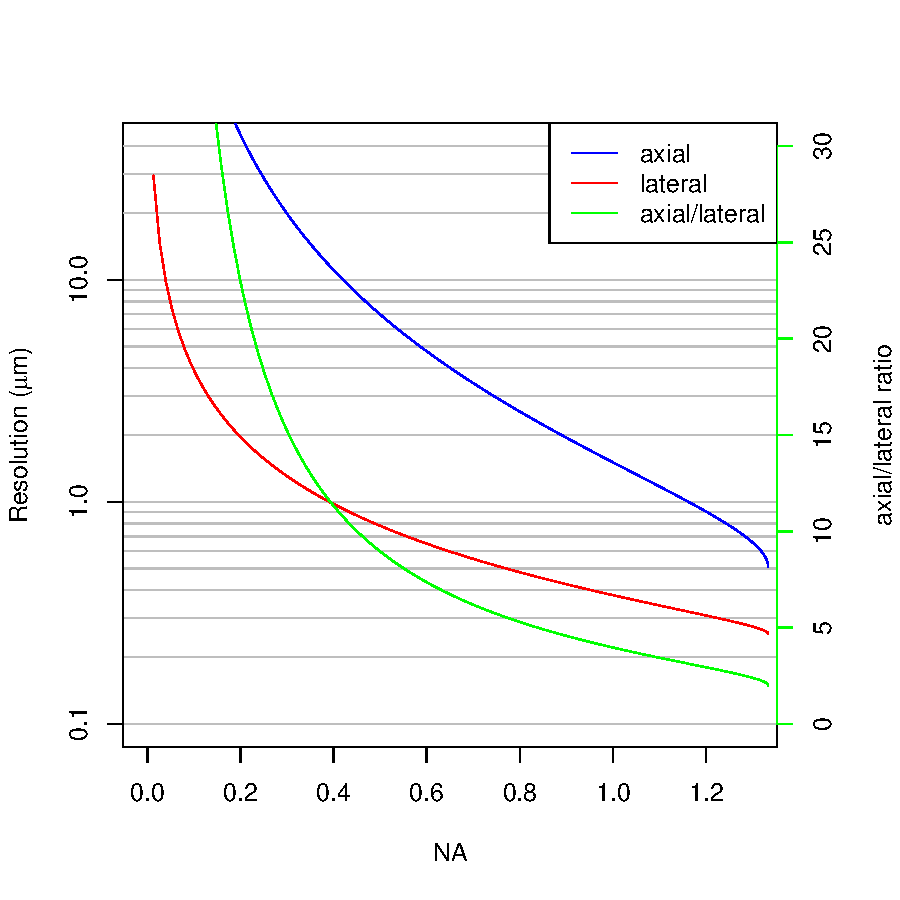
\includegraphics[width=0.6\textwidth]{figures/1_introduction/resolution}
	\caption{\textbf{Resolution of a wide-field microscope.} Axial (blue) and lateral (red) resolutions of a wide-field microscope are shown with respect to the numerical aperture (NA). Resolutions are calculated with $\lambda =510nm$, the emission maximum of GFP and $n=1.333$, the refractive index of water, for water dipping objectives.}
	\label{fig:resolution}
\end{figure}

\section{Confocal microscopy}

Laser scanning confocal microscopy \cite{davidovits_photomicrography_1973} addresses the problem of noise originating from the out of focus planes. The principle for illumination and detection optics is very similar to a wide-filed microscope, but for illumination a focused laser light is used.

The biggest change is in the detection method: the confocal microscope uses a pinhole, to exclude light coming from out of focus planes. Since only those rays are taking part in the imaging that originate from the focus, the image quality is highly improved. This microscopy technique is also capable of 3D imaging, with an axial resolution corresponding to a wide-filed microscope.

However, the image can not be registered as simply as with the wide-filed detection, since at any given time, only a very small portion of the sample will be used in the imaging. Because of this, a more sensitive detection is required, which generally means the use of a photomultiplier. To get the whole image, the focus is scanned through the whole sample (or rather, the sample is scanned through the focus), recording an intensity value for each position. The image is then generated using a computer based on the recorded position and intensity values.


Although this microscopy technique already has 3D capabilities, it's axial resolution is still limited by the SGH theory, since it uses only one objective. Imaging live specimens for an extended period of time with confocal microscopy although possible \cite{aldaz_live_2010}, is not ideal. Since for each voxel imaged, almost the entire specimen has to be illuminated, which results in a very high dose of radiation of the samples. This can be as much as 30--100 times bigger, than the dose used for the actual imaging \cite{reynaud_light_2008}. High power of laser for an extended time frame can result in bleaching the fluorophores, thus resulting in a lower signal at later times, but the more significant issue is phototoxicity, that is when the cells themselves are damaged by the laser light.

\begin{figure}
\begin{subfigure}[t]{0.49\textwidth}
	\centering
	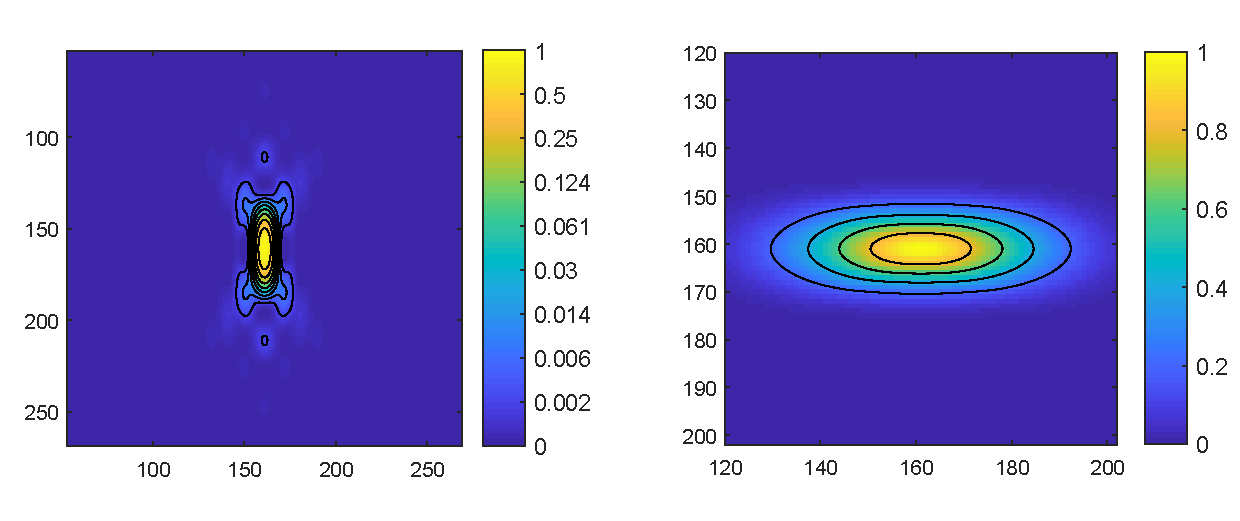
\includegraphics[width=\textwidth]{figures/1_introduction/confocal}
	\caption{\textbf{Confocal microscope}}
	\label{fig:confocal}
\end{subfigure}
\begin{subfigure}[t]{0.49\textwidth}
	\centering
	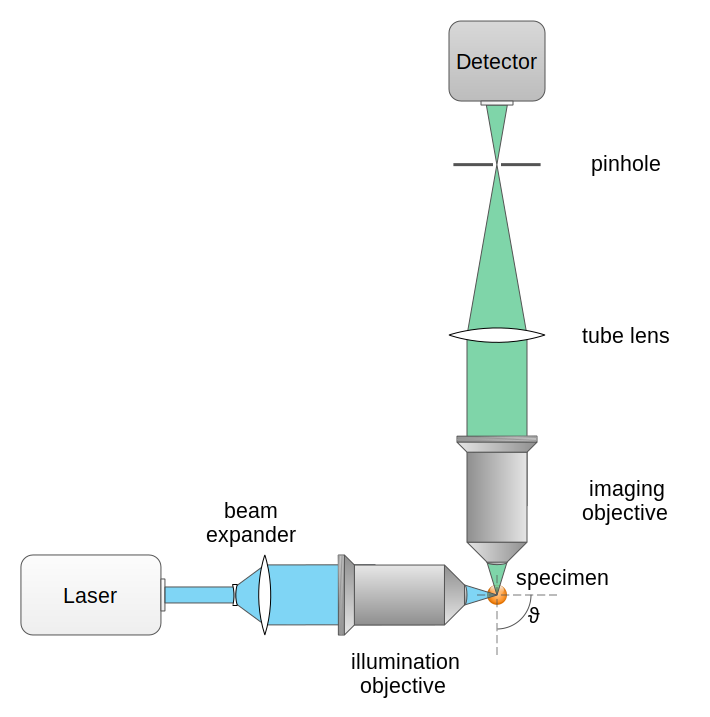
\includegraphics[width=\textwidth]{figures/1_introduction/conf-theta}
	\caption{\textbf{Confocal-theta microscope}}
	\label{fig:conf-theta}
\end{subfigure}
\caption{\textbf{Basic optical components of a laser scanning confocal and confocal-theta microscope.} Both type of microscopes use confocal images detection, which means that a pinhole is used to exclude light coming from out of focus points. Light intensity is measured by a photomultiplier for every voxel in the region of interest. The final image is generated on a computer using the positions and recorded intensity values. A regular confocal microscope (\ref{fig:confocal}) uses the same objective for illumination and detection, while a confocal-theta microscope (\ref{fig:conf-theta}) uses a second objective that is rotated by $\vartheta$ around the focus. In this case, $\vartheta = 90°$.}
\label{fig:confocals}
\end{figure}

\section{Confocal-theta microscopy}

Although confocal microscopy already provides a better resolution in all dimensions, the ratio of the axial and lateral resolution is still very high, due to the single objective illumination and detection. This seriously limits the microscope's 3D imaging capabilities, since in the $z$ direction (i.e. along the imaging axis) the resolution would be significantly worse than in the other directions.

Confocal-theta microscopy \cite{stelzer_fundamental_1994} introduces a second objective to a regular confocal microscope, that is used to illuminate the sample (Figure \ref{fig:conf-theta}). Since this decouples the illumination and detection, using a filter cube is no longer necessary. The second objective is rotated by $\vartheta$ around the focus, this is the where the name of this setup originates.

Resolution is also improved compared to the regular confocal microscope, because the lateral resolution of the imaging objective now corresponds to the axial resolution of the detection objective. The combined resolution of the two-objective system can be calculated in the following manner \cite{krzic_multiple-view_2009}:
\begin{equation}
\frac{1}{\sigma _{sys}^2} = \frac{1}{\sigma _{ill}^2} + \frac{1}{\sigma _{det}^2}
\end{equation}
where $\sigma_{ill} = \sigma_{xy}$ and $\sigma_{det} = \sigma_z$ for the axial resolution of the system, and reversed for the lateral resolution of the system. This means, that the axial and lateral resolution would be the same (if the same objectives are used), and the resulting point spread function is almost isotropic.

Although this is a big improvement to confocal microscopy, the issue of photobleaching and phototoxicity is still not solved with a confocal theta microscope, which means that longer developmental processes are near impossible to follow with this type of microscopy.




\chapter{Single-plane illumination microscopy}
\label{chap2}

The main principle behind single plane illumination microscopy, that is illuminating the sample from the side by a very thin light-sheet, dates back to the early 20\textsuperscript{th} century, when Siedentopf and Zsigmondy first described the ultramicroscope \cite{siedentopf_uber_1902}. This microscope used sunlight as an illumination source, that was guided through a precision slit to generate a thin light-sheet. This allowed Zsigmondy to visualize gold nanoparticles floating in and out of the light-sheet. Since these particles are much smaller than the wavelength of the light, the device was called an ultramicroscope. His studies with colloids together with the development of the ultramicroscope led Zsigmondy to win the Nobel Prize in 1925.

Since then however, light-sheet microscopy was seldom used, but in the last decade it was reinvented and combined with fluorescent microscopy. The first notable light-sheet fluorescent microscope (LSFM) was developed at EMBL in 2004 \cite{huisken_optical_2004}, that demonstrated the benefits of using a light-sheet in imaging developmental processes in three dimension.

Since then, light-sheet based imaging has gained more and more popularity, as it can be adapted and applied to a wide variety of problems. It was numerously proven to be a better choice than confocal microscopy \cite{reynaud_light_2008,huisken_selective_2009} especially in developmental biological applications \cite{weber_light_2011}. It can also be used with a wide variety of specimens of different sizes, such as zebrafish embryo \cite{keller_reconstruction_2008}, mouse brain \cite{dodt_ultramicroscopy:_2007} or drosophila embryo \cite{krzic_multiview_2012}. It is also possible to use light-sheet microscopy in super-resolution, allowing for individual molecule localization \cite{zanacchi_live-cell_2011}.
	
%\begin{itemize}	
%	\item mSPIM, pivoting light-sheet \cite{huisken_even_2007}
%	\item omnidirectional microscopy (review) \cite{weber_omnidirectional_2012}
%	\item SiMView \cite{tomer_quantitative_2012}
%\end{itemize}

\section{Optical properties}

A selective-plane illumination microscope (SPIM) uses a light-sheet to illuminate only a thin section of the sample (Figure~\ref{fig:light-sheet}). This illumination plane is perpendicular to the imaging axis of the detection objective and coincides with the focal plane. This way the image is taken of only that specific plane that is illuminated, thus providing much better signal to noise ratio. In case of conventional wide-field fluorescent microscopy, where the whole specimen is illuminated, light scattering from different regions contribute to a significant background noise. With selective-plane illumination, this problem is intrinsically solved, and it also provides a true sectioning capability. This makes SPIM especially suitable for 3D imaging.



\begin{figure}[htpb]
	\centering
	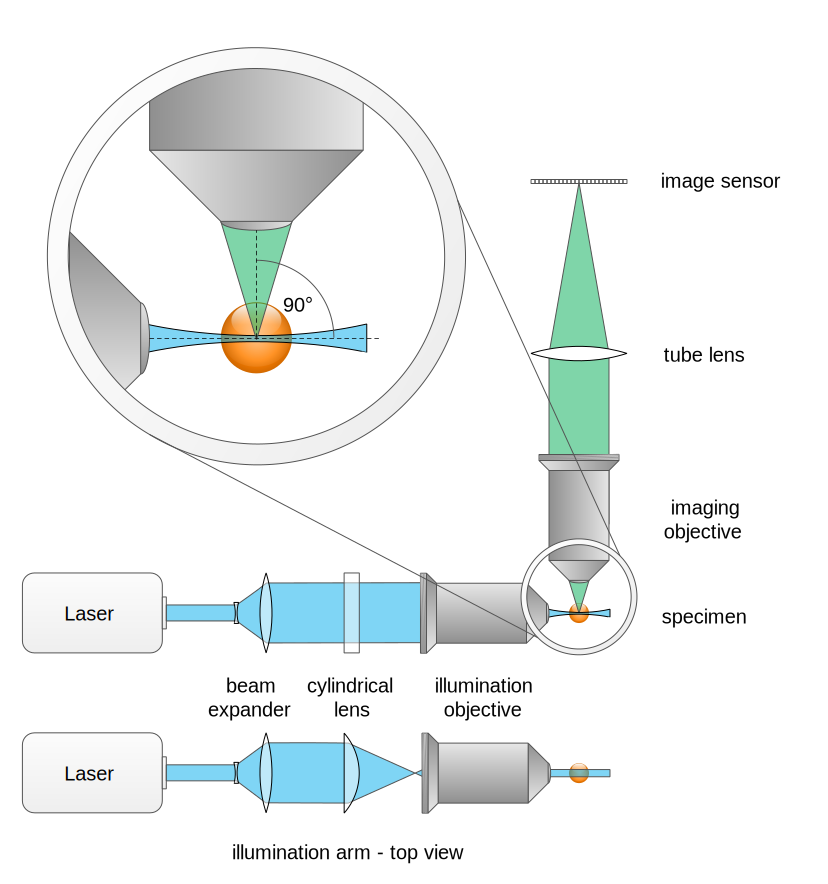
\includegraphics[width=0.8\textwidth]{figures/2_spim/light-sheet}
	\caption{\textbf{Basic optical components of a SPIM.} A selective plane illumination microscope uses two objectives orthogonally aligned. One objective is used to generate a thin light-sheet that illuminates the sample from the side, while the other is used for detection. To generate an image of the specimen, a suitable tube lens is used to focus the light on the sensor of a detection unit (e.g. sCMOS camera). The light-sheet is generated by the illumination objective, using a beam that is previously shaped by a cylindrical lens.}
	\label{fig:light-sheet}
\end{figure}

%\begin{figure}[htpb]
%	\centering
%	\includegraphics[width=0.8\textwidth]{figures/2_spim/sample_holder}
%	\caption{\textbf{Experimental chamber of a LSFM \cite{krzic_multiple-view_2009}.} LSFM is used mostly with water-dipping lenses. The specimen is immersed into a water-based medium contained in a chamber. The chamber has three glass windows, one of them being used for the light-sheet illumination, and the detection objective lens is inserted through a sealing rubber O-ring (shaft seal) in the remaining side. Size of the light sheet is exaggerated.}
%	\label{fig:chamber}
%\end{figure}

%

%The second option to use a virtual light-sheet that is generated by scanning a thin line of laser beam through the sample \cite{weber_light_2011}. If this is done with sufficient speed, a virtual light-sheet will be generated. Since most lasers use Gaussian beams, a light-sheet created by a cylindrical lens will have less intensity towards the edges, which means a wider sheet is needed than the field of view. However, when using the scanning method, the intensity of the virtual light-sheet is uniform through the whole field of view. The disadvantage of this scanning method, is that this scanning motion needs to be very precise, down to the sub-micrometer level to generate a stable virtual light-sheet and this can be hard to achieve.


\subsection{Detection}
The detection unit of a SPIM is basically equivalent to a detection unit of a wide-field microscope, without a dichroic mirror (Figure \ref{fig:light-sheet}). Most important components are the objective together with the tube lens, filter wheel, and a sensor, typically a CCD or sCMOS camera.

One of the most important aspects that determine the resolution of the microscope is the detection objective. Since in developmental biology specimens require a water-based solution, these objectives are usually water dipping objectives directly submerged in the medium. Since the refraction index of water ($n=1.333$) is greater than the refraction index of air, these objectives tend to have a higher $NA$, which results in higher resolution. This, however, also depends on the sensor used, mainly on the pixel size ($d_{sensor}$).

The magnification is typically $10\times$, $20\times$, $40\times$ or $100\times$ but these values are sound only when the objective is used together with the prescribed tube lens. These lenses are specially made to be used with the specific objectives, and are corrected for any aberrations. They typically have a focal length of 160--200mm.

\subsection{Illumination}

\subsubsection{Using cylindrical lens}
The light-sheet can be generated using a cylindrical lens, which focuses the laser beam in only one direction, and creating a thin sheet in the proximity of the focal point. However, to achieve light-sheets that are thin enough, one would need to use cylindrical lens with low focal lengths, but these are hardly accessible in well corrected formats. For this reason, its more common to use a longer focal length cylindrical lens in conjunction with a microscope objective, which is well corrected for chromatic and spherical aberrations \cite{greger_basic_2007}. This way, the light-sheet length, thickness and width can be adjusted for the specific imaging tasks.

For paraxial waves, i.e. waves with nearly parallel wave front normals, a general wave equation can be approximated with the paraxial Helmholz equation \cite{krzic_multiple-view_2009, saleh_fundamentals_2007}
\begin{equation}
	\nabla_T^2 + i 2k \frac{\partial U}{\partial z} = 0
	\label{eq:helmholtz}
\end{equation}
where $\nabla_T^2 = \frac{\partial^2}{\partial x^2} + \frac{\partial^2}{\partial y^2}$, $U(\vec{r})$ is the wave-function, $k=\frac{2\pi}{\lambda}$ is the wavenumber and we assume, that the light spreads in $z$ direction.
 
A simple solution to this differential equation is the Gaussian beam:
\begin{equation}
	U(r,z) = A_0 \cdot \frac{W_0}{W(z)} \cdot e^{-\frac{r^2}{W^2(z)}}\cdot e^{-i\cdot \phi(r,z)}
\label{eq:gaussian}
\end{equation}
where $A_0$ is the amplitude of the wave, $W_0$ is the radius of the beam waist (the thinnest location on the beam), $r=\sqrt{x^2+y^2}$ is the distance from the center of the beam, $W(z)$ is the radius of the beam $z$ distance from the waist, and $\phi(r,z)$ is the combined phase part of the wave-function. Furthermore:

\begin{equation}
	W(z) = W_0\sqrt{1+\left( \frac{z}{z_0} \right)^2}
\end{equation}
where the parameter $z_0$ is called the Rayliegh-range. This has the following connection with the beam waist:

\begin{equation}
	z_0 = \frac{\pi W_0}{\lambda}
\end{equation}
Which means, the thinner the beam waist, the shorter the Rayliegh-range, that is the beam divergence is faster for more focused beams.

Intensity of the emitted flurescence is based on the intensity of the excitation light. In case of a Gaussian beam:
\begin{equation}
	I(r,z) = U(r,z)\cdot U^*(r,z) = |A_0|^2 \cdot \left( \frac{W_0}{W(z)}\right)^2 \cdot e^{-\frac{2r^2}{W^2(z)}}
\end{equation}

Apart from the circular Gaussian beam, the elliptical Gaussian beam is also an eigenfunction of Helmholtz equation (\ref{eq:helmholtz}):
\begin{equation}
	U(x,y,z) = A_0 \cdot \sqrt{\frac{W_{x,0}}{W_x(z)}} \sqrt{\frac{W_{y,0}}{W_y(z)}} \cdot e^{-\frac{x^2}{W_x^2(z)}} \cdot e^{-\frac{y^2}{W_y^2(z)}} \cdot e^{-i\cdot \phi(x,y,z)}
\end{equation}

This beam still has a Gaussian profile along the $x$ and $y$ axes, but the radii are uncoupled, which results in an elliptical beam. Since the beam waist is different along the two axes, the Rayliegh range is also different:
\begin{align}
	z_{x,0} = \frac{\pi W_{x,0}^2}{\lambda} \\
	z_{y,0} = \frac{\pi W_{y,0}^2}{\lambda}
\end{align}
Intensity of the beam is the following:
\begin{equation}
	I(x,y,z) = U(x,y,z)\cdot U^*(x,y,z) = |A_0|^2 \cdot \frac{W_{x,0}}{W_x(z)} \cdot \frac{W_{y,0}}{W_y(z)} \cdot e^{-\frac{2x^2}{W_x^2(z)}} \cdot e^{-\frac{2y^2}{W_y^2(z)}}
\end{equation}
where
\begin{align}
W_x(z) = W_{x,0}\sqrt{1+\left( \frac{z}{z_{x,0}} \right)^2}\mathrm{\quad and \quad } W_y(z) = W_{y,0}\sqrt{1+\left( \frac{z}{z_{y,0}} \right)^2}
\end{align}

Since the illumination is uneven, the usable field of view is smaller than the actual illuminated region (Figure \ref{fig:fov}). The width of the field of view $w_{fov}$ is determined by the Rayliegh length, since this is in a direct relation with the beam divergence. To stay in the optimal region, the light-sheet should only be used in the range of 1 Rayleigh length on both sides of the beam waist (Figure \ref{fig:width}). In this range, the ratio between the thickest (at $z=z_0$) and the thinnest (at $z=0$) part of the beam $W(z)$ will be $\sqrt{2}\approx 1.4142$ which is still acceptable.

Light-sheet height is determined by the profile of the beam along the vertical axis (Figure \ref{fig:height}). Since this is a Gaussian function (see Equation \ref{eq:gaussian}), only a small part in the middle can be used for imaging, because towards the sides the intensity dramatically drops. To allow a maximum 80\% drop of intensity at the edges, the light-sheet height is $h_{fov}=2\cdot 0.472\cdot W_{x,0}$

\begin{figure}[htbp]
	\centering
	\begin{subfigure}[b]{0.7\textwidth}
		\centering
		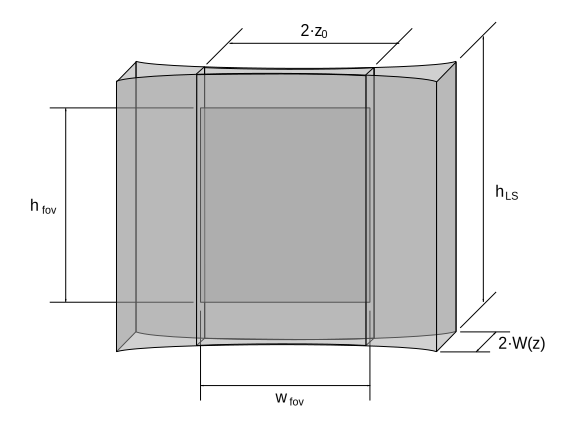
\includegraphics[width=\textwidth]{figures/2_spim/FOV}
		\caption{}
		\label{fig:fov}
	\end{subfigure}
	\begin{subfigure}[b]{0.49\textwidth}
		\centering
		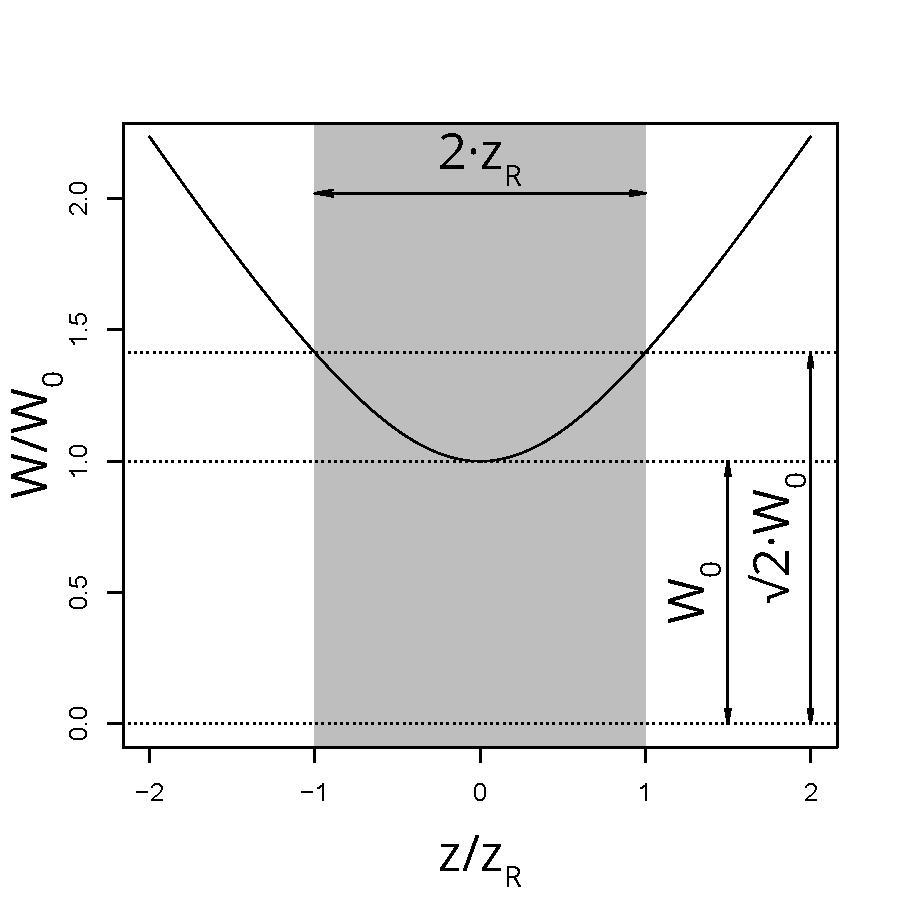
\includegraphics[width=\textwidth]{figures/2_spim/width}
		\caption{}
		\label{fig:width}
	\end{subfigure}
	\begin{subfigure}[b]{0.49\textwidth}
		\centering
		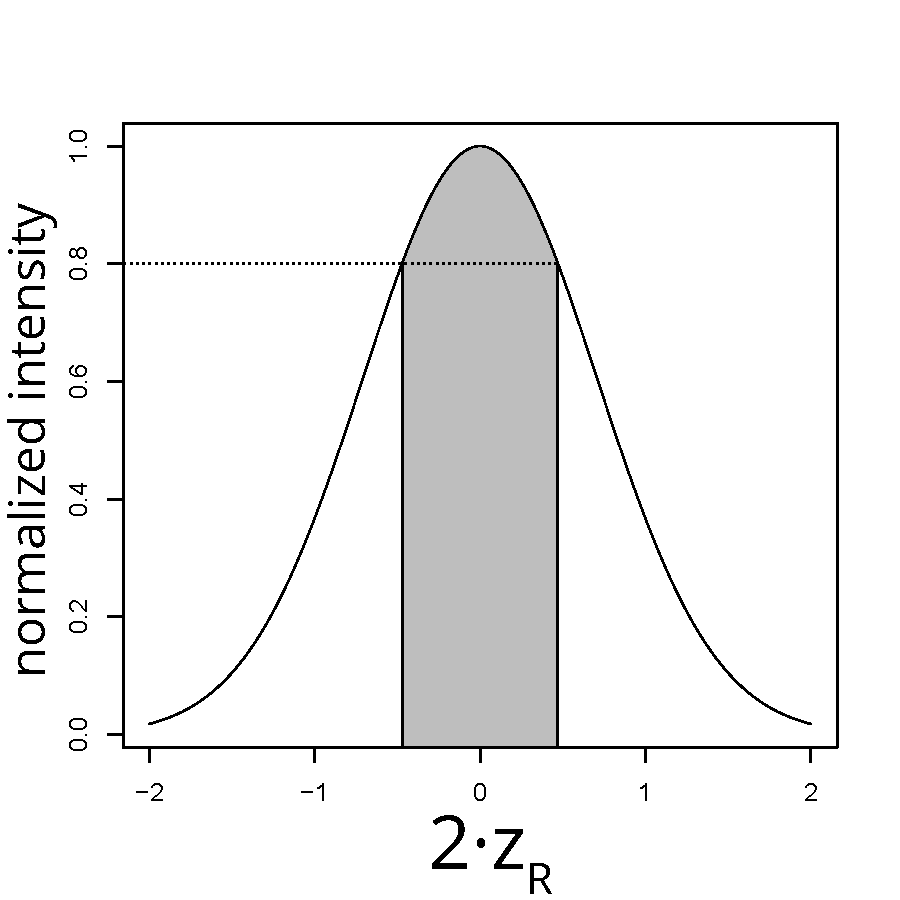
\includegraphics[width=\textwidth]{figures/2_spim/height}
		\caption{}
		\label{fig:height}
	\end{subfigure}
	\caption{\textbf{Light-sheet dimensions.} \ref{fig:fov} shows a light sheet, with the field of view indicated. Since the light-sheet intensity is uneven, the field of view has to be confined to a smaller region. \ref{fig:width} The width and thickness of the field of view depends on the Rayleigh length of the beam ($z_{y,0}$). \ref{fig:height} Height of the field of view is determined by the Gaussian profile of the elliptical beam.}
	\label{fig:ls_dim}
\end{figure}

\subsubsection{Using focused beam scanning}
Since using cylindrical lenses it's not possible to generate a homogeneous light-sheet, moreover at higher magnification the Rayleigh range would be too small, we also consider using focused beam scanning to generate the light-sheet (digital scanned light-sheet microscopy, DSLM). To generate a scanning beam, a galvanometer controlled mirror is used to alter the beam path. This can quickly turn around its axis which will result in an angular sweep with the laser beam. To change the angular movement to translation, a scan lens is used to generate an intermediate scanning plane. This plane is then imaged to the specimen by the tube lens and the illumination objective, resulting in a scanned focused beam.

This method to generate the light-sheet has several advantages compared to a static light-sheet. The height of this sheet is not determined by the cylindrical lens, but it can be dynamically modified. Also, the intensity is uniform through the whole height of the light-sheet.


\begin{figure}[hb]
	\centering
	\includegraphics[width=0.8\textwidth]{figures/2_spim/dslm}
	\caption{\textbf{DSLM illumination.} DSLM illuminates a specimen by a circularly-symmetric beam that is scanned over the field of view. This creates a virtual light-sheet, which illuminates a section of a specimen just like the SPIM. Light-sheet in DSLM is uniform over the whole field of view and its height can be dynamically altered by changing the beam scan range.
}
	\label{fig:dslm}
\end{figure}

\section{Symmetric SPIM}
To address the challenges of isotropic 3D imaging, we propose a new SPIM microscope. Usually, in a SPIM setup, the two objectives have different optical properties -- the one used for imaging typically has a higher NA, and the one used for illumination has a lower NA. In the isotropic SPIM setup we use two objectives of the same type, both for illumination and detection. The objectives are placed in a V-shape, above the sample (Figure~\ref{fig:objectives1}), perpendicular to each other and the light-sheet in a $45^\circ$ angle (Figure~\ref{fig:objectives2}). This arrangement makes sample mounting much easier compared to mounting in capillary, but rotation is not possible.
\begin{figure}[tpd]
	\centering
	\begin{subfigure}[b]{0.49\textwidth}
		\centering
		\includegraphics[width=\textwidth]{figures/2_spim/Image01}
		\caption{Objective alignment}
		\label{fig:objectives1}
	\end{subfigure}
	\begin{subfigure}[b]{0.49\textwidth}
		\centering
		\includegraphics[width=\textwidth]{figures/2_spim/Image04}
		\caption{Light-sheet}
		\label{fig:objectives2}
	\end{subfigure}
	\caption{\textbf{Objective alignment and light-sheet position.}}
	\label{fig:objectives}
\end{figure}

However, since both objectives are used for imaging and illumination in an alternating fashion, this makes sample rotation unnecessary, and images from the two opposing views can be taken in rapid succession. This, and the fact that sample mounting is much simpler makes this microscope an ideal candidate for screening applications. Combined with a multi-positioning stage, it will be possible to image as much as 100 specimens with this microscope.

To achieve this type of operation, it is not enough to just simply put two conventional SPIMs facing towards each other. Since the objectives are now used both for imaging and illumination, a dichroic mirror is needed to couple the optical paths. The dichroic mirror is chosen so it will reflect the wavelength of the illumination light, but transmit the wavelength of the excitation light (Figure~\ref{fig:setup1}). Besides this, the detection uses the same components as a normal wide-field fluorescent microscope, a filterwheel, a tube lens and a detection unit, in our case a CCD camera.
\begin{figure}[htpd]
	\centering
	%\begin{subfigure}[b]{0.8\textwidth}
		\centering
		\includegraphics[width=\textwidth]{figures/2_spim/setup1free}
	%\end{subfigure}
	%\begin{subfigure}[b]{0.8\textwidth}
	%	\centering
	%	\includegraphics[width=\textwidth]{figures/2_spim/setup2free}
	%	\caption{Imaging Branch 2}
	%	\label{fig:setup2}
	%\end{subfigure}
	\caption{\textbf{Schematics of a symmetric SPIM setup.} The laser light is split in two with a 50--50 beamsplitter (BS). The light-paths are selected using mechanical shutters. The laser beam is then shaped using a cylindrical lens (CL), which focuses the beam in one direction to the back focal plane of the illumination objective. This objective then creates the final light-sheet that can be used for imaging. Abbreviations: M -- mirror, BS -- beam splitter, S -- shutter, CL -- cylindrical lens, DM -- dichroic mirror, F -- filter, TL -- tube lens.}
	\label{fig:setup1}
\end{figure}

\subsection{Image registration}
\label{affine}
When imaging with the symmetric SPIM, we have to take into consideration the 45° objective alignment. Since the stage moves horizontally, this will result in a specimen translation not perpendicular to the imaging axis, but rather in a 45° angle. Since normally the 3D image stacks are represented in an orthogonal coordinate system, when displaying a stack made with the symmetric SPIM, it will be sheared along the imaging plane. To correct this, we have to apply an affine transformation, which will align the planes correctly.

When the imaging and translation axes are not perpendicular, but in an $\alpha$ angle, the real stack recorded will be a parallelepiped (Figure \ref{fig:affine}, marked in red). However, when opening it in an image processing application, the program will assume that all the bases are orthogonal, and will display it incorrectly, that is sheared compared to the original, real stack (Figure \ref{fig:affine}, marked in blue).
\begin{figure}[htb]
	\centering
	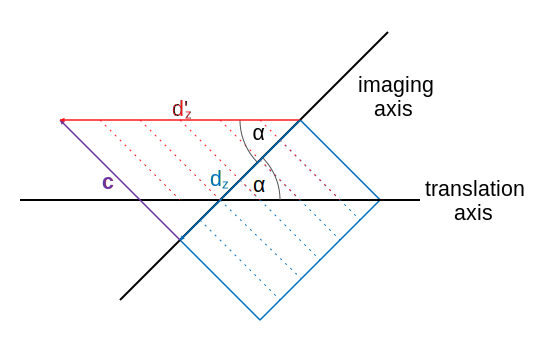
\includegraphics[width=0.8\textwidth]{figures/2_spim/affine}
	\caption{\textbf{Real and virtual stacks.} The red dashed lines indicate the positions where the images are taken. The parallelogram shape is the result of the $\alpha$ angle between the translation and imaging axis. When displaying the stack on a computer, it will display a transformed, virtual stack, which is marked with blue. To correctly display the 3D stack, an inverse of this shear transformation has to be performed.}
	\label{fig:affine}
\end{figure}

To perform the inverse shear transformation, we need to apply the following transformation matrix to our 3D stack:
\begin{equation}
	\mathbf{A}=\begin{pmatrix}
		1 & 0 & 0 \\
		0 & 1 & s \\
		0 & 0 & 1
	\end{pmatrix}
\end{equation}
where $s$ depends on the lateral resolution($d_{xy}$), the stage translation ($d'_z$) and the angle between the imaging and translation axes ($\alpha$).

\begin{equation}
s = \frac{c}{d_{xy}}
\end{equation}
where $d_{xy} = \frac{d_{sensor}}{M}$ and $c=d'_z\cot \sin(\alpha)$, thus
\begin{equation}
s = \frac{d'_z}{\frac{d_{sensor}}{M}} \sin(\alpha) = \frac{d'_z \cdot M}{d_{sensor}} \sin(\alpha)
\end{equation}

For $\alpha = 0°$, when the imaging axis is parallel to the translation axis, $\mathbf{A=I}$.


\chapter{Control unit}
\label{chap3}

Since the microscope setup is custom built and uses components individually selected, the second objective of this work was to develop a program to control and automate image acquisition. The main criteria for this program were modularity and user friendliness. Although the group already had a working microscope (MuVi SPIM \cite{krzic_multiview_2012}) with a custom program, this program was completely specific to that setup. Since the group plans to build several different microscopes that use similar components, we aimed to develop a completely modular program that has the ability to control different SPIM (or other microscope) setups.

User friendliness is also critical, because microscopes are typically used by personnel who has little programming knowledge. To this end, we used LabView to implement the program, because LabView is mainly designed for hardware control it also provides a convenient tool to generate user interfaces.


\section{General description}
The devices we implemented in this program are camera, laser, stage, galvanometric scanner (galvo), filter wheel and shutter. Since most of these devices can be controlled by digital triggers and/or analog signals, and  synchronization is critical, we use an FPGA to generate the appropriate signals. Some devices however are still controlled through other means of communications, such as VISA, through COM port. These devices can introduce some factor of uncertainty, but fortunately all of the devices that are used in the most time-critical operations use digital triggers or analog signals as an input. These devices include the laser, camera, scanning mirror (galvo) and translation stage. Because the program uses these names as class names, in further discussion I will use regular text to refer to physical devices, and emphasized text to refer to \emph{Classes} or \emph{Functions}. For example, laser will mean the actual hardware, and \emph{Laser} will mean the class that is used to control the laser.

When starting the program, the user first has to define the hardware configuration of the microscope. This includes selecting the physical channels the device is connected to and some other parameters that influence how the device should work. These parameters are further discussed in the following sections. After setting up the hardware configuration, it is possible to save the settings and load them later.

When the hardware settings are defined, \emph{Main} loops through each device to initialize them (\emph{InitDevice}). Most of the time this mean opening communication port, handshaking, and setting initial values. In the case of FPGA, this is only setting the initial values. After initialization, \emph{Main} enters the main loop, where it displays the appropriate front panels for devices, listens for user events, and handles them appropriately. Since in the development phase we wanted to have the program as flexible as possible, all devices have a separate front panel, and \emph{Main} opens a new one for each of them. These front panels then communicate with \emph{Main} through TCP/IP, implemented using the STM package for LabView (Figure \ref{fig:program}).

This means, that the user interaction side of the program is completely uncoupled from \emph{Main}, so these front panels could run on a completely different computer. Furthermore, the front panels don't even need to be programmed in LabView, they can be implemented in any other programming language, which makes it possible to run the microscope from a browser for example. TCP/IP communication also enables us to control the whole program through external scripts, without real user interaction. This can be useful in the future for example if we want to couple the microscope operation with real-time image analysis. The external program could adjust the microscope settings according to the results, for example determine the center of mass of the fluorescence, and set the stage so it would be in the center of the field of view.


\begin{figure}[htpb]
	\centering
	\includegraphics[width=0.8\textwidth]{figures/3_program/program}
	\caption{\textbf{Basic structure of the control program.} The main program is written in LabView (National Instruments), and runs on the computer which is directly connected to the components of the microscope. To ensure flexibility and modularity, we took an object oriented approach towards the implementation. The main program only calls the functions of a generic \emph{Device} class, and has no further knowledge of the devices. Black arrows: LabView internal communication; blue arrows: TCP/IP communication.}
	\label{fig:program}
\end{figure}

\section{Detailed operation}
The program is implemented in a way, that the \emph{Main} doesn't need to know anything about the specific data types of the \emph{Devices}. This is achieved through LVOOP (LabView Object Oriented Programming), which is very similar to regular object oriented programming, but still retains the data-flow model used by LabView. The \emph{Main} stores the \emph{Devices} in an associative array, and calls only the high-level functions of the general \emph{Device}. The only exception is the \emph{FPGA} which does need to have some specific functions on \emph{Main}, but this can be treated specially, because it is needed for the operation of several other devices. 

\subsection{Automator}
\label{automator}
The devices apart from the physical components of the microscope, also include an Automator. This Automator is a virtual device, it is used to control the flow of the imaging loop. The two main concepts it uses are Stacks and Channels.

Stacks are used to define a region in the specimen to image. They store two stage positions, a starting and end positions together with the number of planes to image. The \emph{Run} mode will then use this data to move the stage to every position and take an image with the settings specified in Channels.

A Channel defines the settings of every device that is used to by the microscope, except for the stage (stage data is used in Stacks. When the user is satisfied with a certain combination of settings, e.g. laser wavelength and intensity, filter type or exposure time; they can define a Channel based on the current device settings. These Channels then can be added to the Stacks, even to multiple Stacks, or multiple Channels to the same Stack.

\begin{figure}[htbp]
	\centering
	\includegraphics[scale=0.5]{figures/3_program/automator2}
	\caption{\textbf{User interface for Automator.} The front panel of the Automator consists of 3 main panels. The left panel contains a library of possible commands or functions that define the flow of microscope automation. The center plane displays further information when an element is chosen from the library, and the right panel shows the Scheduler, which contains the currently selected operations. Adding elements to the queue can be done simply by drag-and-drop, and they can be removed or modified by right clicking on them. When in run mode, the execution status is displayed next to the elements (green).}
	\label{fig:ui_automator}
\end{figure}

\subsubsection{Live mode}
\label{automator:live}
In live mode, all the front panels are active, the user can interact with the devices in real time, and see the result immediately. This mode is used to move the specimen to the correct positions, define stacks and find the optimal settings for channels. Live mode has two further options, continuous and single. Depending on the user's choice, the images are taken continuously, or just on at a time. Continuous mode offers faster feedback on the changes, and so this is normally used for coarse alignment of the specimen, or adjusting the light-sheet properties. Single mode is better suited for sensitive samples. Using this to fine-tune the settings although can take a little more time, but the phototoxic stress on the sample is greatly reduced.

Live mode is also used to define the flow of the automated image acquisition. Once the stacks and channels are defined, the user can build a command queue of these elements (see Figure \ref{fig:ui_automator}). The simplest case uses a loop over time: one can specify the delay between the loops and the number of repetitions. This feature can be used for time-lapse imaging. 

Other options are also taken into consideration, but are not yet implemented. This could include for example some kind of checkpoint, where after taking the images they are immediately processed (either in LabView, or an other application), and depending on the results, the settings of the microscope could be updated automatically.


\subsubsection{Run mode}
When the user defines the flow of the microscope program and clicks on Play, the Automator will enter the Run mode. Here, a series of functions will be called based on the scheduler queue. Once the next element in the queue is executed it is removed, unless it is tagged, in which case it will be popped back to the queue again. This is the case for the stacks for example.

If the stacks would just run in a loop with a pre-set number of repetitions, aborting or stopping the execution would not be so simple. In this case however, when a stack is running and the user clicks Pause or Stop, these command will be pushed in the queue before the next stack. This means, that the program flow can be easily manipulated while it is still running.
 
When executing the time loop, the \emph{Automator} loops through all the stacks (all of them are represented in the scheduler queue), and then in a stack loops through all channels. Before executing a stack, $PreStack$ is called, which sets the stage to its initial position and calls any other functions that need to run before taking the stack. After this, the \emph{Automator} loop through all the channels that are defined for the stack, and after completing this it calls \emph{PostStack} for all devices which prepares the devices to be ready for the next stack.

Executing the channels also consists of 3 parts: \emph{PreChannel}, \emph{Execute}, and \emph{PostChannel}. The pre- and post functions serve similar functions as the ones for the stacks, only this is on a different level of execution, thus allowing for more generalized structure. After setting every device to the appropriate initial position defined in the channel, the \emph{Automator} loops through all the planes and performs stage translation, laser control and image exposure in a synchronized fashion. Since all the devices that are used at this point receive signals from the FPGA, this part of the program just uploads the appropriate commands on the card and executes them.


\subsection{FPGA}
\label{fpga}
FPGA, or field programmable gate array is an integrated circuit device that can be reconfigured after manufacturing. Since the reprogramming is done in the hardware level, FPGAs can be really fast executing a single, specific operation. They usually also provide configurable inputs and outputs which can be used for measurements or to control other devices.

To program the FPGA we used the FPGA module for LabView, which creates an interface to the FPGA that enables normal vi-s (virtual instruments) to communicate with the FPGA and pass data to it. The card we use is NI PCIe-7841R, which contains a Xilinx Virtex-5 LX30 FPGA. It has 8 analog and 96 digital outputs, and the current version uses 8 of each. The digital outputs have a maximum output rate of 40MHz, while the analog outputs have a maximum output rate at 1MHz. Output ranges from -10 V to 10 V with 16 bit resolution. These properties make this FPGA card especially useful when generating the signals to control time-critical operations.

\subsubsection{Sections}
We define a signal with a series of sections that are interpreted by the FPGA. For the digital lines these sections are defined by a section length, section value which is a boolean value, and section type. Since the FPGA operates in discrete time domain, instead of continuous time, we define the length of a signal in counter ticks ($n=t/f$, where $f$ is the counter frequency on the FPGA and $t$ is the signal length). Section type is also boolean, it defines whether to update the output to a new value, or use the previous one. In this case, section value is not taken into consideration, only the section length (Figure \ref{fig:sections}).

For analog channels the section value is a 16 bit integer which will be converted to voltage in the range of -10 V to 10 V. Analog sections have two more properties: Dvalue and DDvalue, which are values of the first and second derivative respectively. For every time point, the FPGA integrates, and adds the DDvalue to the Dvalue, and Dvalue to the value, which becomes the output signal. Section type is also different, it is a 1D boolean array of length 3, which defines if the value, Dvalue or DDvalue needs to be updated or not at the beginning of the section.

\begin{figure}[htbp]
\centering
\begin{subfigure}[b]{0.49\textwidth}
		\centering
		\begin{tabular}{r|c|c|c}
		%\hline \hline
			& 1 & 2 & 3 \\ \hline \hline
	length  & 100 & 100 & 200 \\
	value   & 0 & 10000 & 0 \\
	Dvalue  & 0 & -200 & 0 \\
	DDvalue & 0 & 0 & 1 \\
	type (base 2) & 111 & 011 & 110 \\
	\multicolumn{4}{c}{ }\\ %\hline \hline
\multicolumn{4}{c}{ }\\ %\hline \hline
\end{tabular}
		\caption{}
	\end{subfigure}	
	\begin{subfigure}[b]{0.49\textwidth}
		\centering
		\includegraphics[width=0.8\textwidth]{figures/3_program/sections}
		\caption{}
	\end{subfigure}
\caption{\textbf{Example for analog sections.} The first section sets every value to 0, resulting in a constant signal for 100 ticks. The next section then sets only the value and Dvalue, to 10000 and -200 respectively, this produces a linear slope. The last section sets the Dvalue and DDvalue to 0 and 1, which results in a parabolic signal that starts from the last value of the previous section.}
\label{fig:sections}
\end{figure}


Using these sections to define the signals is very convenient, since the data passed to the FPGA is minimal compared to the case where all the values are calculated for every time point. Instead, we just need to send these few parameters, and the FPGA will do the calculations for any signal that can be represented as a series of linear and parabolic segments.

The FPGA also uses a global variable which is the signal length in ticks. After the number of iterations reach this number, the FPGA sets all channels back to the initial position and starts iterating form the beginning again. This length is the sum of the exposure time and the delays that the user defined. If the sections for a channel are shorter than this signal length, then the sections will repeat periodically until the signal length is reached.

\subsubsection{Uploading new sections}

Whenever the device settings change in \emph{Main}, the program recalculates the sections and sends this data to the FPGA through a FIFO, which enables direct memory access on the FPGA. The sections for every 8 channel are sent as a continuous stream of numbers, but at the beginning of every channel the first value indicates the number of sections that the channel will need to use. Also, before all the sections, the length of the whole data stream is sent, so the FPGA will know right away how much data it will need to handle.

Based on this number, the FPGA then reads the values and stores them in an internal random access memory block. When executing the sections, the pointer to the first element of the sections are specified, and the FPGA will iterate through all of them sequentially. Since the memory on the FPGA is big enough, it is possible to upload multiple streams of sections, each of them to a different starting position of the memory block. After this is done, the $Main$ just needs to send the appropriate pointer value, and the FPGA will execute the corresponding sections.

Another feature of the FPGA program, is the automatic smooth transition of analog signals when new sections are uploaded to the card that has different initial values than the current values. This is necessary, because in some cases the analog signal directly controls a mechanical system that can be very sensitive to sudden changes of the input. Although some of these devices has built in low-pass filters to prevent this, it is still better not to take the chance, and use smooth transitions whenever possible. 

These transitions are achieved also by using sections to define paraboloids, but in this case the FPGA itself calculates these based on its current state and the next initial values. These sections are then stored in a separate part of the memory, so the \emph{Main} can not modify it. The transition occurs immediately after uploading the new sections, this way ensuring that the outputs are already in the correct initial position when starting executing the sections.

\subsubsection{Section manager}
\label{section_manager}
Since the instruments controlled by the FPGA are not completely independent, we introduced a section manager that collects data from all the devices and synchronizes their settings. In some cases for example, when a device needs a parabolic output, it can happen that when calculating the sections for these devices, the sum of their length won't be exactly the same as the globally defined length. This happens due to rounding errors, and even though the ratio of these error are quite small ($<10^{-3}$), they can not be neglected. At first, this won't pose any problems, but since these section run periodically again and again, the different channels will go out of synchronization which will severely affect the imaging quality.

The section manager deals with this problem in a way, that if it detects that under the current setting a timing error would occur, it overrides the section lengths for those devices that don't use any rounding when calculating the sections. Even though this will result in a slightly different timing than the user specified, the ratio of difference as mentioned, in below $10^{-3}$, so the overall image quality won't be affected.

The section manager also has the ability to qualitatively change the behaviour of a device. The laser for example has two modes of operation, one with galvo and one without it. For more details see sections Laser (\ref{laser}) and Galvo (\ref{galvo}).

\begin{figure}[htbp]
	\centering
	\includegraphics[scale=0.5]{figures/3_program/fpga}
	\caption{\textbf{User interface for FPGA.} In this interface the user can specify all the timing values of an imaging cycle, including the exposure time and delays before and after exposure. Values have to be provided in milliseconds. When in live mode (see Automator, section \ref{automator:live}) the user can also control the trigger output using the Live and Single buttons.}
	\label{fig:ui_fpga}
\end{figure}
\subsubsection{User interface}
The FPGA settings can be modified through a specific front panel (Figure \ref{fig:ui_fpga}). Since most of the other devices depend on the FPGA, especially those used for the actual imaging, the timing has to set here. This includes setting an exposure time, and a delay before and after the exposure. The reason we have 2 different delays instead of just one, is that this solution offers more flexibility when designing the triggers of an imaging cycle.

The front panel also has two buttons, Live and Single. When the microscope is in live mode (i.e. started but not acquiring images), the FPGA by default doesn't send any triggers yet. The user can control the trigger output by turning Live on or off on the FPGA front panel. Turning this on will start sending triggers to all connected devices continuously. To offer a better control, when Single is selected and turning Live on, the FPGA will send only one period of the triggers instead of a continuous signal. This allows the user to have a more precise control over the amount of laser used, which can significantly reduce photobleaching effects occurring while setting up the experiment.

Additional to the settings above, one can also specify the length of the smooth transition that occurs when updating the analog sections on the FPGA.



\subsection{Camera}
Cameras are handled on a different computer (see Figure \ref{fig:program}) for two reasons. First, compared to the other devices, they have significantly more options, and thus it requires more elaborate programming to control them. Even though most cameras share some basic settings, they can be very different depending on the manufacturer. Because of this, the \emph{Camera Control} program is completely separate from the \emph{Main}, and uses a simple command-based communication over TCP/IP. This approach allows us to easily expand the range of supported cameras by just implementing the appropriate functions for this command-based operation.

The other reason to have the cameras on a different computer is that they produce such incredible amount of data in a short period of time, that serious computing power is needed just to store the images. To ensure smooth operation, this process needs to be handled on a different computer than the one that runs \emph{Main}. The dedicated camera computer generally has more RAM (typically 24 GB), and uses a RAID 0 array of up to 7 hard drives.

\begin{figure}[htbp]
	\centering
	\includegraphics[scale=0.5]{figures/3_program/camera}
	\caption{\textbf{User interface for camera}}
	\label{fig:ui_camera}
\end{figure}

The user interface has two parts: one runs on the main computer, while the other on the dedicated camera computer. The program on the main computer (Figure \ref{fig:ui_camera}) is really simple. It only has two options, a button to reconnect to the camera computer in case the connection was lost, and a switch to select whether to use the camera for imaging or not. This function is useful when using the program with more than one cameras (such as in case of the symmetric SPIM), but we don't need both to image at the same time.

The program on the camera computer differs with each type of camera, but the structure is the same. After initializing the camera, and connecting to \emph{Main} through TCP/IP, the camera program starts three parallel loops.

The first loop has three states, and it defines the camera operation mode. These can be idle, continuous image acquisition or finite image acquisition. Idle mode is self explanatory, continuous mode is used when the \emph{Main} is in live mode, while finite is used when imaging a stack, since in this case the number of images to acquire are predefined.

The second loop constantly listens for user interactions on the camera program front panel. These include for example setting the ROI or the binning of the camera, along with some camera specific setting, such as operating mode of the sensor, camera cooling, or trigger mode.

The third loop listens to the \emph{Main} through the TCP/IP communication, and performs the appropriate functions, acknowledging completion by replying to the command. These commands include for example getting camera settings, initializing directory structure, or starting finite image acquisition. In most of the cases, when the camera completed the action, it just replies with "Done", however in the case of getting the camera settings, it also sends a user readable string that contains the most important settings along with all of the setting flattened to a string. The \emph{Main} uses the user readable string to display it in the \emph{Automator} window, but has no knowledge how to interpret the full settings. These settings are just stored in the appropriate channel data, and before starting to image a stack, they are sent back to the camera control computer which can interpret it, and will set the camera accordingly.


\subsection{Laser}
\label{laser}
The lasers are controlled through a digital and an analog channel simultaneously. The analog channel sets the laser power, while the digital channel controls the blanking. The input typically ranges from 0--1 V to 0--5 V based on the laser model. When configuring a new laser for the program, one has to provide this range together with the channels used by the FPGA, and the wavelength of the laser. The user has the option to configure up to 6 laser lines which will share the same front panel (Figure \ref{fig:ui_laser}).

\begin{figure}[htbp]
	\centering
	\includegraphics[scale=0.5]{figures/3_program/laser}
	\caption{\textbf{User interface for laser}}
	\label{fig:ui_laser}
\end{figure}
The front panel is dynamically generated based on the current laser configuration. The number of controls appearing depends on the laser lines configured, and each of these controls are colored based on the wavelength specified. On the laser on/off button the wavelength is also displayed in numbers for easy identification.

Each laser line has several options, but the most important is the on/off switch and the slider to set the power. The number on this slider shows the intensity output in percentage of the maximum power. Although usually the laser triggers have to be synchronized with the camera triggers, in some cases this might not be enough. For example, in STED (stimulated emission depletion microscopy) \cite{hell_breaking_1994} a series of different laser pulses are used before the actual imaging. To this end, we implemented an override function which can be enabled separately for each laser line. When this option is enabled, the laser line will use its own timing information that can be set to any desired value.


Operating the laser through \emph{Main} is rather simple, each channel only requires 3 sections (Table \ref{tab:laser}). The timing for both the analog and digital channels are the same, each defined by the \emph{FPGA} settings exposure ($n_{exp}$), delay before ($n_{d_1}$) and delay after ($n_{d_2}$). These sections use constant values, so Dvalue and DDvalue remains 0 for all of them. The only thing that varies is the value, during exposure the digital trigger is high, and the analog line sets the voltage corresponding to the required output power.

The laser has a second operation mode, depending on the system configuration. If the microscope uses a galvo to generate a virtual light-sheet, the laser pulses are synchronized with the linear movements of the galvo (see Galvo, section \ref{galvo}).

\begin{table}[htb]
\centering
\begin{subfigure}[h]{0.49\textwidth}
\centering
\begin{tabular}{r|c|c|c}
		%\hline \hline
			& 1 & 2 & 3\\ \hline \hline
	length  & $n_{d_1}$ & $n_{exp}$ & $n_{d_2}$ \\
	value   & 0 & 1 & 0  \\
	type  & 1 & 1 & 1\\
\end{tabular}
\caption{Digital sections}
\end{subfigure}
\begin{subfigure}[h]{0.490\textwidth}
\centering
\begin{tabular}{r|c|c|c}
		%\hline \hline
			& 1 & 2 & 3\\ \hline \hline
	length  & $n_{d_1}$ & $n_{exp}$ & $n_{d_2}$ \\
	value   & 0 & $I$ & 0  \\
	Dvalue  & 0 & 0 & 0 \\
	DDvalue & 0 & 0 & 0 \\
	type    & 111 & 111 & 111 \\
\end{tabular}
\caption{Analog sections}
\end{subfigure}
\caption{\textbf{Sections used by \emph{Laser}.} Laser output is defined in 3 sections on both analog and digital channels. A digital channel is used to enable or disable laser blanking, while the analog signal sets the laser intensity. Note that for the analog channels, only one section would be sufficient that stores the intensity, since the digital line controls on/off state. Abbreviations: $n_{d_1}$: delay length before exposure, $n_{exp}$: exposure length, $n_{d_2}$: delay length after exposure, $I$: laser intensity.}
\label{tab:laser}
\end{table}




\subsection{Galvo}
\label{galvo}

A galvo, or galvanometer-driven laser scanning mirror is used to generate the virtual light-sheet for the microscope. This is controlled through an analog channel quite simply: the galvanometer turns a mirror attached to it based on the input voltage. Although modern galvos can scan with a high speed, up to 1000 Hz, they are very delicate instruments, and one has to be careful when operating them. This was one of the main reasons why we implemented the smooth transition function on the FPGA (see section \ref{fpga}).

To achieve an evenly illuminated light-sheet, the scanning has to be done linearly, and more than once if possible during the exposure. Generally this would be achieved by a triangle signal, but in the case of the galvo we can't use it. Because the signal is translated to a mechanical movement, and its derivative at the turning point is not continuous, this would mean an infinite acceleration for the galvo. To avoid this, and avoid damaging the instrument, we use short parabolic segments at the turning point.


\begin{table}[phtb]
\centering
\begin{tabular}{r|c||c|c|c|c|c|c||c}
		%\hline \hline
			& 0 & $6n+1$ & $6n+2$ & $6n+3$ & $6n+4$ & $6n+5$ & $6n+6$ & $6N+1$ \\ \hline \hline
	length  & $n_{d_1}$ & $n_1$  & $n_2$ & $n_1$ & $n_1$ & $n_2$ & $n_1$ & $n_{d_2}$ \\
	value   & $A+U_0$   & $A+U_0$& 0     & 0     & 0     & 0     & 0     & $A+U_0$       \\
	Dvalue  & 0         & 0      & $v$   & 0     & 0     & $v$   & 0     & 0         \\
	DDvalue & 0         & $a$    & 0     & $-a$  & $-a$  & 0     & $a$   & 0         \\
	type    & 111       & 111    & 110   & 100   & 100   & 110   & 100   & 111       \\
\end{tabular}
\caption{\textbf{Analog Sections used by Galvo.} The sections can be divided in 3 parts: delay before exposure, exposure and delay after exposure. The first (0) and last ($6N+1$) sections represent the delays, while the others are used to generate the scanning motion. One scan is again divided into 6 sections: acceleration, linear, deceleration and the same in the opposite direction. $n\in \{1, 2, ... , N-1\} \subset \mathbb{N}$, where $N$ is the number of scans performed during an exposure. Note that at the beginning of each scan, the value is also reset to the initial position. Even though the FPGA uses 48 bit upsampling when calculating the sections, some rounding errors can still occur, especially for faster transitions. Setting the initial value at the beginning of a scan counteracts the accumulating error. $n_{d_1}$, $n_{d_2}$: length before and after exposure, $n_1$: length of acceleration/deceleration, $n_2$: length of linear section, $v$: slope of the linear section, $a$: acceleration, $A$: amplitude, $U_0$: offset}
\label{tab:galvo}
\end{table}

\begin{figure}[phtb]
	\centering
	\includegraphics[width=0.7\textwidth]{figures/3_program/triggers}
	\caption{\textbf{Signals sent to devices when a galvo is used.} The signals displayed use the following timing settings: exposure time: 50ms, delay: 50ms, turn time percentage: 32\%, scan amplitude: 0.02V, number of scans: 2. Laser triggers are synchronized with the galvo scanning: the laser is only on, when the galvo is in a linear section. This ensures even illumination through the whole field of view. Camera triggers are unaffected. Turn time percentage is exaggerated for demonstration purposes, typically  10\% is used.}
	\label{fig:triggers_galvo}
\end{figure}

One scanning period consists of 6 parts (Table \ref{tab:galvo} and Figure \ref{fig:triggers_galvo}). The first three corresponds to acceleration, linear scanning and deceleration. The second three are very similar, only in the opposite direction. The turn time can be controlled by the user, by changing the turn time percentage parameter on the front panel (Figure \ref{fig:ui_galvo}). This is a percentage of the exposure time that will be used for turning the galvo. Since in this time the galvo movement is not linear, the laser is switched off to avoid uneven illumination at the sides. This synchronization is done by the Section manager of the \emph{FPGA} (see FPGA, section \ref{section_manager}).

\begin{figure}[htbp]
	\centering
	\includegraphics[scale=0.5]{figures/3_program/galvo}
	\caption{\textbf{User interface for galvo} The following parameters can be changed: scanning amplitude, offset, number of scans and turn time percentage.}
	\label{fig:ui_galvo}
\end{figure}

\subsection{Stage}
To position the sample, a piezoelectric translation stage is used. Depending on the configuration, the stage can use 1, 2 or 3 translation axes. The micro-controller of this device uses an analog input signal in the range of 0--10V, and positions the stage between its boundaries accordingly. Every axis has its own input signal, each coming from its own channel on the FPGA.

During the hardware configuration, the number of axes has to be specified along with the channel number and the direction (this is only needed for displaying). Each axis also needs a lower and upper boundary, specified in $\mu m$. Finally, the user has to provide the scaling factor from $\mu m$ to Volt, so the FPGA will use the correct values.

Through the front panel (Figure \ref{fig:ui_stage}) the user can move the stage to different positions using the arrow buttons for X and Y direction, and the $+$ and $-$ signs for Z direction. The step can be specified in the DXYZ field. Apart from interacting with the buttons, one can directly specify the position value in the X, Y and Z fields in $\mu m$. These values will be coerced to the physical boundaries of the device, which was given during the hardware configuration.

\begin{figure}[htbp]
	\centering
	\includegraphics[scale=0.5]{figures/3_program/stage}
	\caption{\textbf{User interface for stage.} The arrow, $+$ and $-$ buttons can be used to move the stage by the value specified in DXYZ. It is also possible to directly write the new position in the fields X, Y or Z. A stack is defined by setting the starting and end position using the SetStart and SetEnd buttons, and specifying the number of planes. The user interface adapts itself to the stage configuration, allowing to change only those axes that were previously defined. This illustration only uses the X axis.}
	\label{fig:ui_stage}
\end{figure}

This front panel is also used to define the Stacks (see Automator, section \ref{automator}). One can specify the starting and end position of the stage, and the number of images to take. Based on these values, the front panel automatically displays the distance between the planes, so the user has a better feedback. It is also possible to reverse a stack, which is useful when imaging with multiple channels. In principle it is possible to link more channels to the same stack, but in that case when the first channel is ready, the stage will move back again to the starting position. If the user specifies two stacks for the two channels, both between the same positions but in the opposite direction, the jumping will not occur.

While in run mode, in the \emph{PreStack} phase, a single stack is uploaded to the FPGA with the starting position of the stage. This will smoothly move the stage to the correct position using the automatic smooth transition feature of the \emph{FPGA}. Since this section will never run actually, its length is irrelevant, so we just use a length of one tick.

Once the \emph{Main} enters the \emph{Execute stack} function, the stage will use 3 sections for the translation movement (Table \ref{tab:stage}). For the time of the first delay and the exposure the stage will stay in the same positions, and during the second delay the stage will move to the next position. This movement consists of two parts, an acceleration and a deceleration, so there will be no jumps. In each section only the DDvalue is updated, all other values are taken from the previous sections. To compensate for unlikely but possible rounding errors, the first section also sets the Dvalue to 0. This makes sure, that the stage will stay in the same position for the whole exposure time.

\begin{table}[htbp]
\centering
\begin{tabular}{r|c||c|c|c}
		%\hline \hline
			& 0 & 1 & 2 & 3\\ \hline \hline
	length  & 1 & $n_{d_1} + n_{exp}$ & $n_{d_2}/2$ & $n_{d_2}/2$ \\
	value   & $U_{0}$ & 0 & 0 & 0  \\
	Dvalue  & 0 & 0 & 0 & 0 \\
	DDvalue & 0 & 0 & $a$ & $-a$ \\
	type    & 111& 110 & 100 & 100 \\
\end{tabular}
\caption{\textbf{Analog sections used by the stage.}}
\label{tab:stage}
\end{table}



\subsection{Filter wheel}
The filter wheels used by our group communicate through a COM port, via the VISA communication protocol. When setting up the microscope's hardware configuration, one has to specify the COM port, and based on the filter wheel model, also the wheel to use. These can accommodate 6 to 10 filters. During the hardware setup the filter types can be specified in an array of strings, with the array index corresponding to the filters physical position in the wheel.

While in live mode, the front panel (Figure \ref{fig:ui_fw}) shows a drop-down list containing the previously specified filter names. Changing the value immediately takes effect, because this device is not controlled by the FPGA.

During imaging, the filter wheel is only used in the \emph{PreChannel} function, where it is set to the correct position specified by the current channel setting.

\begin{figure}[htbp]
	\centering
	\includegraphics[scale=0.5]{figures/3_program/fw}
	\caption{\textbf{User interface for filter wheel} The front panel show a drop-down list with the available filter names. Using this, the user can specify the filter to be used for imaging.}
	\label{fig:ui_fw}
\end{figure}



\subsection{Shutter}
A shutter is a mechanical device that can move in and out of the laser's illumination path. Using this device it is possible to switch between the illumination and imaging path.

The devices we use require a digital input, 0 meaning an open shutter and 1 meaning closed. To control this device, the FPGA only needs one section, a section with the length of an imaging cycle ($n_{d_1}+n_{exp}+n_{d_2}$), and a value to determine the state. The user can change the state on the front panel (Figure \ref{fig:ui_shutter}), and also has the possibility to set a waiting time in seconds. This should correspond to the time the shutter needs to switch between the states. Before executing a stack the shutter is set to the correct position and the program waits for it to complete movement before starting the imaging.

Although this is the simplest device of all, it can be versatilely used with other devices also. Instead of a shutter for example, it is possible to use this class to control a flipping mirror. Such mirror can be used to alter the laser path, which can also be used to switch between different illumination paths.

\begin{figure}[htbp]
	\centering
	\includegraphics[scale=0.5]{figures/3_program/shutter}
	\caption{\textbf{User interface for shutter} The simplest device only have two options: a button to choose whether the shutter is open or closed, and a delay specified in seconds. This delay is used in the run mode: before starting to take the images the program will wait for the shutter to perform the movement.}
	\label{fig:ui_shutter}
\end{figure}







\chapter{Results}
\label{chap4}

In this chapter I will describe the symmetrical SPIM we built based on the principles discussed in Chapter \ref{chap2}, and present some images that were acquired using the program described in Chapter \ref{chap3}.

\section{Microscope setup}
The setup is built on a Melles Griot optical table that uses Newport laminar-flow isolators as legs. The optical components are mounted on a 65 mm rail system. To achieve symmetric imaging two identical objectives (O1 and O2 on Figure \ref{fig:photo}) are placed perpendicular to each other and 45° to the table. The objectives are mounted on custom designed turrets, that are compatible with the rail system. Both turrets have a mechanical translation stage coupled to the objectives which can be used to align the focus. One of the turrets has an additional horizontal translation stage, which adds a third degree of freedom to position the objectives. Both objectives are water-dipping, $40\times$ magnification with 0.8 numerical aperture.

\begin{figure}[htbp]
	\centering
	\includegraphics[width=\textwidth]{figures/4_results/photo2}
	\caption{\textbf{Symmetrical SPIM.} Illumination light path shown in blue, fluorescence light path shown in green. The translation stage was taken out to allow a better view on the objective alignment. Abbreviations: O1, O2: objectives, SM: scanning mirror, SL: scan lens, BS: beam splitter, TL: tube lens, FM: flip mirror, EF: emission filter}
	\label{fig:photo}
\end{figure}

For illumination an Omicron LightHub\textsuperscript{\textregistered}-6 laser combiner is used, which houses a \mbox{405 nm}, 488 nm, 561 nm and 647 nm lasers. The output is coupled to the microscope using fiber optics.

To record the images of the two objectives, the system uses two identical Hamamatsu ORCA-Flash4.0 sCMOS cameras. These cameras have a resolution of $2048 \times 2048$, pixel size of 6.5 $\mu m$, and can acquire images at 100 fps on full resolution. Readout noise and quantum efficiency is also exceptionally good.

Light-sheet is generated by scanning with the focused laser-beam using a galvanometer-driven scanning mirror (SM). To make sure that the illumination paths are as identical as possible, the beam is split only after the scanning mirror, immediately after the scan lens (SL). This is done by a 50-50 beam splitter (BS). After the beam splitter, both illumination arms have a 160 mm tube lens (TL) that focuses the beams on the back focal plane of the objectives. The other focus of these lens coincide with the focus of the scan lens. To separate the illumination and imaging paths, a flip mirror (FM) is used to reflect the illumination light towards the objectives.

To use an objective for imaging, the corresponding flip mirror is opened, and this will allow the light coming from the objective to pass through to the imaging tube lens. This lens will then focus the light on the detector of the camera (not shown on the image).

The imaging path also contains an emission filter (EF), to separate the illumintaion and fluorescence light. In this case, since for the first time we only imaged using a single channel, these are fixed filters, a filter wheel is not used.



\section{3D imaging}
First we used the microscope to image \textit{Phallusia mammillata}, or white sea squirt embryo. \textit{Phallusia m.} is a chordate intervertebrate model organism for developmental biology. Although phylogenetically this species is rather far from humans, it's widely used when studying embryogenesis, since it has relatively small amount of cells, and it is very transparent \cite{ettensohn_methods_2004}. This property is especially useful in imaging, using SPIM very clear images can be obtained of these embryos.

Since \textit{Phallusia m.} is a sea creature, imaging is also performed in seawater. Labelling is done using the fluorescent dye FM4-64, which attaches to the cell membrane and has a quite broad emission and absorption spectrum \cite{bolte_FM-dyes_2004}. The embryos were attached to glass plates mounted on the stage, submerged in seawater. For imaging we used 488 nm laser, 50 ms exposure time and 2 $\mu$m translation. Because of the 45° arrangement, this resulted in a  $\sqrt{2}\ \mu m$ distance between the planes.

After taking a stack, it was affine transformed, to reverse the shear effect of the 45° translation (see Image registration, section \ref{affine}) using the open source application Fiji \cite{schindelin_fiji:_2012}. The result is shown on Figure \ref{fig:ph1}.


\begin{figure}[htbp]
	\centering
	\includegraphics[width=0.8\textwidth]{figures/4_results/phallusia_montage2}
	\caption{\textbf{Z-sections of a \textit{Phallusia mammillata} embryo.} Cell membranes are dyed with FM4-64 fluorescent marker. Excitation wavelength: 488 nm, exposure time: 50 ms, distance between planes: 1.4142 $\mu m$, magnification: $40\times$. Every 6\textsuperscript{th} image is shown.}
	\label{fig:ph1}
\end{figure}

\section{Time-lapse imaging}

To test the stability of the system, we imaged the same \textit{Phallusia m.} embryo for 4 hours, every 2 minutes using the same setting as described before. All the images were acquired, and the specimen stayed in the same position. After affine transforming all of the stacks, we generated a 3D projection of each using Fiji. These projections are then used as frames in a time lapse movie. Figure \ref{fig:ph2} shows every 5 frame of this movie.

\begin{figure}[htbp]
	\centering
	\includegraphics[width=0.8\textwidth]{figures/4_results/phallusia_montage_time2}
	\caption{\textbf{Time-lape imaging of \textit{Phallusia mammillata} embryo.} The same embryo was imaged with a 488 nm excitation laser using 50 ms exposure time. Images were acquired every 2 miutes, for 4 hours. Figure shows 3D projections of every 10 minutes.}
	\label{fig:ph2}
\end{figure}

\section{Confocal imaging with light-sheet microscopy}
It was recently shown, that using Hamamatsu sCMOS cameras it is possible to combine light-sheet microscopy with line-scanning confocal microscopy \cite{baumgart_scanned_2012}. In this setup, the scanning of the laser is synchronized with the camera readout, thus excluding side-scattered light from imaging. However, to achieve this type of imaging, one has to use a rolling shutter instead of a global shutter. This means, that exposure of the chip is done row by row with a slight delay, and readout is also done in the same manner after some integration time. Depending on when the readout starts, one can set the width of this virtual slit.

To test if our setup would also benefit from this kind of image registration, we imaged a \emph{Drosophila melanogaster} embryo that expressed mCherry histone marker. Since implementing the rolling shutter mode, and synchronizing it with the scanning wasn't the objective of this project, we imaged the specimen illuminated with a single beam at different positions and merged the images in Fiji to simulate the slit mode.

The embryo was illuminated with a 561 nm laser, using 20 ms exposure time and 20 ms delay. The embryo was fully covered with 85 different positions of the beam, so imaging took 3.4 seconds. After acquiring the images, the images were fused using two different methods. First, the images were simply averaged, with this representing the global shutter mode (Figure \ref{fig:ds_avg}). In the second method before averaging, we applied a non-linear filter to all of the frames, this way simulating the effect of the slit (Figure \ref{fig:ds_max}).

\begin{figure}[tbp]
	\centering
	\begin{subfigure}[b]{0.49\textwidth}
		\centering
		\includegraphics[width=\textwidth]{figures/4_results/ds_avg}
		\caption{}
		\label{fig:ds_avg}
	\end{subfigure}
	\begin{subfigure}[b]{0.49\textwidth}
		\centering
		\includegraphics[width=\textwidth]{figures/4_results/ds_max}
		\caption{}
		\label{fig:ds_max}
	\end{subfigure}
	\caption{\textbf{Drosophila melanogaster embryo.} Images were taken of a single beam in different positions and fused later using two different methods. \ref{fig:ds_avg} shows the result of a simulated global shutter mode, while \ref{fig:ds_max} shows the result of a simulated rolling shutter mode. The rolling shutter results in a much clearer image with less scattering and more contrast.}
	\label{fig:ds}
\end{figure}

Difference between the two images is striking. The image simulating the rolling shutter mode has significantly less scattering, higher contrast and overall better image quality. This image registration method would be especially useful when imaging opaque samples (such as \emph{Drosophila m.}), but more transparent samples would also benefit from the better contrast. 

\section{Discussion}
Single plane illumination microscopy is a rapidly growing part of optical microscopy. It's use of a thin illumination plane to excite fluorophores is much more efficient than the scanning method of confocal microscopy. Since the method uses two objectives in a perpendicular alignment, the axial resolution of the system is greatly improved. Fast imaging and low illumination power makes this technique especially useful when investigating developmental biological processes, such as early embryo development.

In this work, I summarized the basic principles of selective plane illumination microscopy, and took part in developing a symmetrical SPIM system, that is designed to operate on high speeds, and offers near isotropic 3D images through image fusion.

Moreover, a custom program was developed in LabView, which enables easy control and automation of the microscope setup, as well as other similar setups. The program was ultimately tested on three different microscopes, using rather different hardware configurations, and in all three cases it performed above expectations.

Using this program, and the prototype of the symmetrical SPIM, we imaged a live \textit{Phallusia m.} embryo for an extended time, and showed, that despite the lack of rotation, dense specimens, such as \textit{Drosophila m.} embryos can also be imaged with high quality if using a (simulated) rolling shutter exposure mode.

Further plans for this microscope include implementing the rolling shutter mode for enhanced image quality, adding real-time image processing capabilities for automatic self-calibrating, and adding a multi-positioning stage for possible screening applications. 

\newpage
\cleardoublepage
\phantomsection
\begin{acknowledgements}

I would like to thank Lars Hufnagel for this opportunity to work in his group, and involving me in developing this microscope system. He gave me a lot of support, and helped in understanding and solving the possible difficulties that we came across during the development process.

I greatly appreciate the help of Uroš Kržič, who gave me an insight on the principles of selective plane illumination microscopy, and also prepared some illustrations for this work.

I thank Stefan Günther for providing the \textit{Drosophila m.} embryos, and \mbox{Ulla-Maj} Fiuza for providing the \textit{Phallusia m.} embryos.

Finally, I would like to thank Gustavo Quintas Glasner de Medeiros and Nils Norlin, as they both participated in the microscope design and program development, and both of them inspired me greatly. Without their help, I couldn't have written this paper.

\addcontentsline{toc}{chapter}{Acknowledgements}
\end{acknowledgements}

\cleardoublepage
\phantomsection
\addcontentsline{toc}{chapter}{References}
\bibliographystyle{IEEE/IEEEtran}
{ \footnotesize \bibliography{tdk}}


\end{document}
